\documentclass[a4paper,11pt]{article}

\usepackage{fullpage} % Package to use full page
\usepackage{parskip} % Package to tweak paragraph skipping
\usepackage{amsmath}
\usepackage{hyperref}
\usepackage{amsmath,amsfonts,amsthm} % Math packages
\usepackage{graphicx}
\usepackage{listings}
\usepackage{caption}
\usepackage{subcaption}
\usepackage{color}
\usepackage{float}
\definecolor{codegreen}{rgb}{0,0.6,0}
\definecolor{codegray}{rgb}{0.5,0.5,0.5}
\definecolor{codepurple}{rgb}{0.58,0,0.82}
\definecolor{backcolour}{rgb}{0.95,0.95,0.92}
\definecolor{brown}{rgb}{0.59, 0.29, 0.0}
\definecolor{beaublue}{rgb}{0.74, 0.83, 0.9}
\definecolor{orange}{rgb}{1.0, 0.5, 0.0}
\definecolor{darkslategray}{rgb}{0.18, 0.31, 0.31}
\def\Xint#1{\mathchoice
	{\XXint\displaystyle\textstyle{#1}}%
	{\XXint\textstyle\scriptstyle{#1}}%
	{\XXint\scriptstyle\scriptscriptstyle{#1}}%
	{\XXint\scriptscriptstyle\scriptscriptstyle{#1}}%
	\!\int}
\def\XXint#1#2#3{{\setbox0=\hbox{$#1{#2#3}{\int}$}
		\vcenter{\hbox{$#2#3$}}\kern-.5\wd0}}
\def\dashint{\Xint-}

% Swap the definition of \abs* and \norm*, so that \abs
% and \norm resizes the size of the brackets, and the 
% starred version does not.
\makeatletter
\let\oldabs\abs
\def\abs{\@ifstar{\oldabs}{\oldabs*}}
%
\let\oldnorm\norm
\def\norm{\@ifstar{\oldnorm}{\oldnorm*}}
\makeatother
\definecolor{keywords}{RGB}{255,0,90}
\definecolor{comments}{RGB}{0,0,113}
\definecolor{red}{RGB}{160,0,0}
\definecolor{green}{RGB}{0,150,0}
\definecolor{codegreen}{rgb}{0,0.6,0}
\definecolor{codegray}{rgb}{0.5,0.5,0.5}
\definecolor{codepurple}{rgb}{0.58,0,0.82}
\definecolor{backcolour}{rgb}{0.95,0.95,0.92}
\definecolor{brown}{rgb}{0.59, 0.29, 0.0}
\definecolor{beaublue}{rgb}{0.74, 0.83, 0.9}
\definecolor{orange}{rgb}{1.0, 0.5, 0.0}
\definecolor{darkslategray}{rgb}{0.18, 0.31, 0.31}
\definecolor{deepblue}{rgb}{0,0,0.5}
\definecolor{deepred}{rgb}{0.6,0,0}
\definecolor{deepgreen}{rgb}{0,0.5,0}
\lstdefinestyle{myMatlabstyle}{
	language=Matlab,
	backgroundcolor=\color{white},   
	commentstyle=\color{codegreen},
	keywordstyle=\color{blue},
	identifierstyle=\color{brown},
	numberstyle=\tiny\color{codegray},
	stringstyle=\color{orange},
	basicstyle=\footnotesize,
	breakatwhitespace=false,         
	breaklines=true,                 
	captionpos=b,                    
	keepspaces=true,                 
	numbers=left,                    
	numbersep=5pt,                  
	showspaces=false,                
	showstringspaces=false,
	showtabs=false,                  
	tabsize=2
}
\lstdefinestyle{myPythonstyle}{
	language=Python, 
	basicstyle=\ttfamily\small, 
	keywordstyle=\color{blue},
	commentstyle=\color{green},
	stringstyle=\color{red},
	showstringspaces=false,
	identifierstyle=\color{black},
}
\lstset{language=Matlab,frame=single}
\lstset{language=Python,frame=single}

\title{AMATH 575: Problem Set 3}
\author{Jithin D. George, No. 1622555}
%\date{23/11/16}
% matrix environment
\newenvironment{mat}{\left[ \begin{array}{ccccccccccccc}}{\end{array}\right]}
\newcommand\bcm{\begin{mat}}
	\newcommand\ecm{\end{mat}}

\begin{document}

\maketitle
\begin{enumerate}

	

	\item
	This nifty code aids us in plotting the Goodwin equation in time.
	\begin{lstlisting}[style=MyPythonstyle]
import numpy as np
from scipy import integrate
import matplotlib as mpl
from mpl_toolkits.mplot3d import Axes3D
import matplotlib.pyplot as plt
def Goodwin(X,t):
	return X[1], -0.75*((X[0]**2-1)/(X[0]**2+1))*X[1]+\\
	0.5*X[0]-0.5*X[0]**3 +14*np.sin(t)
fig = plt.figure()
ax = fig.gca(projection='3d')
circa =np.linspace(0,2*np.pi,1000)
index=0
plotspace1= np.zeros((1000,2))
for i in circa:
  a_t = np.arange(0, 4*np.pi, 0.01)
  asol = integrate.odeint(Goodwin, [np.cos(i),np.sin(i)], a_t)
  plotspace1[index,:]=asol[-1,:]
  index +=1    
  ax.plot(a_t,asol[:,0],asol[:,1])
plt.show
	\end{lstlisting}
The first two iterates are plotted below.
\begin{figure}[H]
	\centering
	\begin{subfigure}{.5\textwidth}
		\centering
		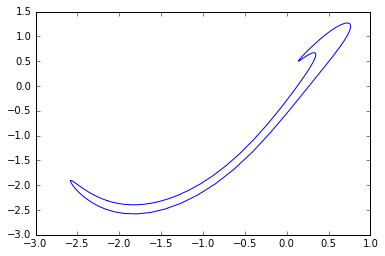
\includegraphics[width=\linewidth]{firstiter}
		\caption{The first iteration}
		\label{fig:sub1}
	\end{subfigure}%
	\begin{subfigure}{.5\textwidth}
		\centering
		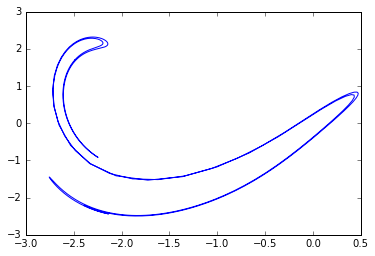
\includegraphics[width=\linewidth]{seconditer}
		\caption{The second iteration}
		\label{fig:sub2}
	\end{subfigure}
	\caption{The first two iterations}
\end{figure}
This code generates a 3-dimensional plot in (y,y',t) phase. 
\begin{figure}[H]
	\centering
	\includegraphics[width=10cm]{Goodwin}
	\caption{The 3-d plot with time as the third axis}
\end{figure}
	\item
	\[A = \bcm a & b \\ c &d \ecm\]
	\[A^TJA=J\]
	\[ \bcm a^T & c^T \\ b^T &d^T \ecm \bcm 0& I \\ -I &0 \ecm\bcm a & b \\ c &d \ecm = \bcm 0& I \\ -I &0 \ecm\]
	\[ \bcm   -c^T & a^T\\ -d^T & b^T  \ecm \bcm a & b \\ c &d \ecm = \bcm 0& I \\ -I &0 \ecm\]
	\[ \bcm a^Tc-c^Ta & a^Td-c^T b \\ b^Tc-d^Ta &b^Td-d^Tb \ecm = \bcm 0& I \\ -I &0 \ecm\]
	\begin{enumerate}
		\item
	Thus, we see 
	\[a^Tc-c^Ta =0, b^Td-d^Tb=0 \] 
	For this to work, $a^Tc$ and $b^Td$ have to be symmetric.
	\item
	We also see that 
	\[a^Td-c^T b =I\]
	\item
	 An attempt at the solution
	\[det(A)= det(ad - bc)=det(a^Td-c^Tb) = det(I)=1\]
	I was unable to show the middle step: det(ad - bc)=det($a^Td-c^Tb$) .
\end{enumerate}
	
	
	
	\item
	Assume there are two symplectic transformations. One between ($q_1,p_1$) and ($q_2,p_2$) and another between ($q_2,p_2$) and ($q_3,p_3$). Our goal is to prove the transformation between ($q_1,p_1$) and ($q_3,p_3$) is symplectic.
	The Jacobian A of that transformation is given by 
	\[A = \bcm \frac{\partial q_3}{\partial q_1} & \frac{\partial q_3}{\partial p_1} \\ \frac{\partial p_3}{\partial q_1} & \frac{\partial p_3}{\partial p_1}\ecm= \bcm \frac{\partial q_3}{\partial q_2}\frac{\partial q_2}{\partial q_1} + \frac{\partial q_3}{\partial p_2}\frac{\partial p_2}{\partial q_1} & \frac{\partial q_3}{\partial q_2}\frac{\partial q_2}{\partial p_1} + \frac{\partial q_3}{\partial p_2}\frac{\partial p_2}{\partial p_1} \\ \frac{\partial p_3}{\partial q_2}\frac{\partial q_2}{\partial q_1} + \frac{\partial p_3}{\partial p_2}\frac{\partial p_2}{\partial q_1} & \frac{\partial p_3}{\partial q_2}\frac{\partial q_2}{\partial p_1} + \frac{\partial p_3}{\partial p_2}\frac{\partial p_2}{\partial p_1}\ecm\]
	\[=\bcm \frac{\partial q_3}{\partial q_2} & \frac{\partial q_3}{\partial p_2} \\ \frac{\partial p_3}{\partial q_2} & \frac{\partial p_3}{\partial p_2}\ecm \bcm \frac{\partial q_2}{\partial q_1} & \frac{\partial q_2}{\partial p_1} \\ \frac{\partial p_2}{\partial q_1} & \frac{\partial p_2}{\partial p_1}\ecm \]
	\[= A_2 A_1\]
	
	Where $A_1$ and $A_2$ are the Jacobians for the first two transformations.
	\[A^TJA=(A_2 A_1)^TJ(A_2 A_1)= A_1^T A_2^T J A_2 A_1 =A_1^T J A_1 = J  \]
	
	Thus, the composition of two symplectic transformations is sympletic.
	\item 
	\begin{enumerate}
		\item
		The Jacobian of a Hamiltonian is a infinitesimal symplectic matrix. So, if the jacobian has an eigenvalue $\lambda$, then $-\lambda$ is also an eigenvalue. Thus, there would be no fixed point with only negative eigenvalues. Thus, an asymptotic fixed point is not possible.

		\item
		If the jacobian of a Hamiltonian vector field has an eigenvalue $\lambda$, then $\bar{\lambda}$ is also an eigenvalue. Also, if 0 is an eigenvalue, it has even multiplicity. Thus, because of this, there is no way to obtain a center manifold of odd dimensions.
		


	\end{enumerate}	
	
	\item 
	
	If the trace of the Jacobian of a system is zero, it is volume preserving.
	Thus, the following matrix B is volume-preserving since it has no diagonal elements.
	\[B  = \bcm  0 &0 &0 &1\\ 1 &0 &0 &0\\ 0 &0 &0&1\\ 0 &0 &1 &0 \ecm\]
	\[B^T + JB = \bcm  0 &0 &0 &2\\ 0 &0 &1 &0\\ 0 &-1 &0&-1\\ -2 &0 &1 &0 \ecm \]
	So, this is definitely not a Hamiltonian vector field.
	Thus, the following vector field is volume preserving and not Hamiltonian.
	\[x_1' = x_4\]
	\[x_2' = x_1\]
	\[x_3' = x_4\]
	\[x_4' = x_3\]
	\item
	\begin{enumerate}
		\item
		\[q_1' = p_1\]
		\[ q_2' = - p_2\]
		\[ p_1' = \lambda q_1 - 3\phi^2 q_1 - q_2\]
		\[ p_2' = -\lambda q_2 + \phi^2 q_2 - q_1\]
	
		\item
		The Jacobian B is given by

		
		\[B = \bcm 0 &0 &1 &0\\ 0 &0 &0 &-1\\ \lambda -3\phi^(x)&-1 &0 &0\\ -1 &\phi^(x)-\lambda &0 &0 \ecm\]
		\[B^TJ+JB= \bcm 0 &0 &\lambda-3\phi^2(x) &-1\\0 &0 &-1 &\phi^2(x)-\lambda\\1 &0 &0 &0\\ 0 &-1 &0 &0\ecm \bcm 0 &0 &1 &0\\0 &0 &0 &1\\ -1 &0 &0 &0\\ 0 &-1 &0 &0 \ecm  \]
		\[+  \bcm 0 &0 &1 &0\\0 &0 &0 &1\\ -1 &0 &0 &0\\ 0 &-1 &0 &0 \ecm \bcm 0 &0 &1 &0\\ 0 &0 &0 &-1\\ \lambda -3\phi^(x)&-1 &0 &0\\ -1 &\phi^(x)-\lambda &0 &0 \ecm\]
		\[= \bcm -(\lambda-3\phi^2(x)) &1 &0 &0\\1 &\lambda -\phi^2(x) &0 &0\\ 0 &0 &1 &0\\ 0 &0 &0 &-1 \ecm +\bcm (\lambda-3\phi^2(x)) &-1 &0 &0\\-1 &-\lambda +\phi^2(x) &0 &0\\ 0 &0 &-1 &0\\ 0 &0 &0 &1 \ecm\]
		
		\[= 0\]
		Thus,$B^TJ +JB =0$ seems to hold.
		\[H = \int_{0}^{1}<f(tx),Jx>dt\]
		\[ = \int_{0}^{1}\bcm t p_1 \\ - t p_2\\ \lambda  t q_1 - 3\phi^2(x)  tq_1 -  tq_2\\ -\lambda t q_2 + \phi^2(x)t q_2 - tq_1  \ecm . \bcm p_1\\ p_2\\-q_1 \\ -q_2\ecm dt\]
		\[ = \int_{0}^{1}t( p_1^2 - p_2^2-\lambda (q_1^2+q_2^2) + 3\phi^2(x) q_1^2 +\phi^2(x) q_2^2 -2q_1q_2 )dt \]
		\[ H =  \frac{1}{2}(p_1^2 - p_2^2-\lambda (q_1^2+q_2^2) + 3q_1^2 \phi^2(x)   +q_2^2 \phi^2(x) +2q_1q_2)  \]
		\[\frac{\partial H}{\partial p_1}= p_1= q_1'\]
		\[\frac{\partial H}{\partial p_2}= -p_2= q_2'\]
		\[\frac{\partial H}{\partial q_1}= -\lambda q_1 +3 q_1 \phi^2(x)  +q_1 = -p_1'\]
		\[\frac{\partial H}{\partial q_2}= -\lambda q_2 +3 q_2 \phi^2(x) +q_1  = -p_2' \]
		Thus, there exists a Hamiltonian too.
		
		So, the Homotopy theorem seems to hold in this case.
		
		\item
		Using Mathematica,
		\[\frac{dH}{dx}= p_1p_1' - p_2p_2' -\lambda(q_1q_1'+ q_2q_2')+ 3q_1q_1'\phi^2(x)+3q_1^2\phi(x)\phi(x)' \]\[+ q_2q_2'\phi^2(x)+q_2^2\phi(x)\phi(x)' +2q_1'q_2+2q_2'q_1\]
		\[= 3q_1^2\phi(x)\phi(x)' + q_2^2\phi(x)\phi(x)'\]
		
		Thus, since it is non-autonomous, the Hamiltonian is not a first integral.
		
		\item
		\[q_1' = q_2\]
		\[ q_2' = \lambda q_1 - 3\phi^2 q_1 - p_1\]
		\[ p_1' = p2\]
		\[ p_2' = \lambda p_1 - \phi^2 p_1 + q_1\]
		Here, the Jacobian is given by 
		\[B=\bcm 0 &1 &0 &0\\\lambda - 3\phi^2 &0 &-1 &0 \\0 &0 &0 &1 \\1 &0 &\lambda - \phi^2 &0 \ecm \]
		\[B^TJ +JB \text{ is not zero} \]
		This is not zero (shown in the last Mathematica attachment). So, it is not infinitely symplectic.
		\[H = \int_{0}^{1}<f(tx),Jx>dt\]
		\[ = \int_{0}^{1}\bcm t q_2 \\ t(\lambda q_1 - 3\phi^2 q_1 - p_1) \\   t p_2\\ t(\lambda p_1 - \phi^2 p_1 + q_1)  \ecm . \bcm p_1\\ p_2\\-q_1 \\ -q_2\ecm dt\]
		\[=(1-\lambda+\phi^2(x)) p_1q_2 +\lambda q_1p_2 -3\phi^2 q_1p_2 - p_1p_2 -p_2q_1 -q_1q_2\]
		\[\frac{\partial H}{\partial p_1} \text{ is not } q_1'\]
		Thus, the Homotopy operator does not yield a Hamiltonian.
	\end{enumerate}
	\item
	All these are done in the Mathematica attachment.
	\begin{enumerate}
		\item
		Here, we split things up to real and imaginary parts and we show that $B^TJ +JB =0 $
		
		\item
		Here, we show that the two transformation are equivalent using the Expand function and equating them.
		\item
		Here, we equate the derivative of the Hamiltonian and make sure that it matches with $q_1', p_1'$ etc.
		
		
	\end{enumerate}	
	 
	\item 
	\[ x' = \alpha x - \beta xy \]
	\[ y' = \delta xy -\gamma y \]
	The conserved quantity V for the Lotka-Volterra model is given by
	\[V = -\delta x + \gamma ln(x)- \beta y + \alpha ln(y)\]
	Let's see if it's a Hamiltonian under the coordinates (q,p)--(ln(x),ln(y)).
	\[ H= -\delta e^q + \gamma q- \beta e^p + \alpha p\]
	\[ q' = \frac{\partial H}{\partial p}= - \beta e^p + \alpha \]
	\[ \frac{1}{x}x' = - \beta y + \alpha\]
	\[x' =  \alpha x - \beta x y\]
	\[ q' = -\frac{\partial H}{\partial q}= \delta e^q - \gamma \]
	\[ \frac{1}{y}y' = \delta x - \gamma\]
	\[ y' = \delta x y - \gamma y\]
	Thus, we can recover the original system and our conserved quantity is a Hamiltonian
	
	
	


	\end{enumerate} 
\end{document}